\documentclass[11pt,twocolumn,DIV=11]{scrartcl}

\usepackage{amsmath}
\usepackage{framed}
\usepackage{color}
\definecolor{shadecolor}{gray}{0.8}

\usepackage{natbib}
\bibliographystyle{apalike}

\usepackage{tikz}
\usetikzlibrary{bayesnet}

\renewcommand\phi\varphi
\DeclareMathOperator*{\argmax}{arg\,max}

\author{
    Verdegaal, Jacob\\
    \texttt{jacob.verdegaal@student.uva.nl}
    \and
    Drumm, Eli T.\\
    \texttt{etd@dte.li}
    \and
    Noble, Bill\\
    \texttt{winobes@gmail.com}
}

\title{Inducing Semantic Frames on a Very Large Corpus of Syntactic-Ngrams}

\begin{document}

\maketitle


\section{Introduction}
Here we provide some background information about what are semantic frames and 
what it menas to induce them and stuff like that.


\section{Related Work}
Here we talk mostly about the O'Connor paper \citep{oconnor2013} and the Rooth 
paper \citep{rooth1999}.


\section{Induction Models}

We consider two probabalistic latent-variable models that learn semantic frames
from verb-subject-object tripples (VSO's).
The goal of these models is to use th syntactic information give by a VSO to
infer what kind of event it describes (i.e., to which semantic frame it belongs).

\subsection{Model 0}

The approach models each VSO independenly, without considering any further context.
Word distributions are completely independent between arguments and accross frames.
Tuples are clustered according to which frame's three distributions best fit the 
three arguments.

\begin{figure}

    \begin{snugshade}
    \scriptsize
    For each $i = 1..N$:\\
    \hspace*{15pt} Draw a frame $f \sim \theta$.\\
    \hspace*{15pt} Draw a verb $v \sim \phi_f^v$\\
    \hspace*{15pt} Draw a subject $s \sim \phi_f^s$\\
    \hspace*{15pt} Draw an object $o \sim \phi_f^o$
    \end{snugshade}

    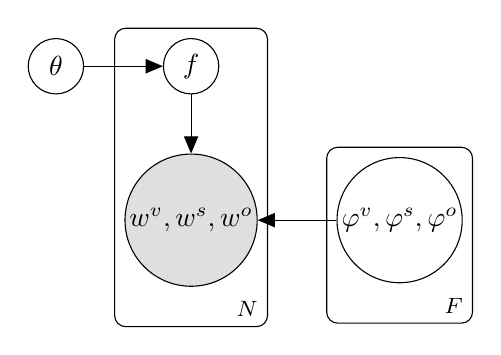
\begin{tikzpicture}
  % Nodes
  \node[obs] (datapoint) {$w^v,w^s,w^o$} ; %
  \node[latent, above=0.75cm of datapoint] (F) {$f$} ; %
  \node[latent, left=of F] (theta) {$\theta$}; %
  \node[latent, right=of datapoint] (phi) {$\varphi^v,\varphi^s,\varphi^o$}; %
  \edge {theta} {F} ; %
  \edge {F} {datapoint}
  \edge {phi} {datapoint} ; %
  \plate {tuples} {(F) (datapoint) } {$N$}; %
  \plate {} {(phi)} {$F$} ; %
\end{tikzpicture}


    \caption{Model 0 generative story}
    \label{gen0}

\end{figure}

Model 0 is based on one originally proposed in \citet{rooth1999}, which 
considers noun-verb pairs. Following \citet{oconnor2013}, we expand the model
to use the limited syntax of VSOs.

The generative story (figure \ref{gen0}) gives us the following joint probability:
\begin{align*}
&P(\mathbf{f},\mathbf{w}|\phi,\theta) 
  = P(\mathbf{f}|\theta)P(\mathbf{w}|\phi)\\
  =& \prod_{i=1}^{N}\big[\theta(f_i) \prod_a^{\{v,s,o\}}\phi_{f_i}^a(w_i^a)\big]
\end{align*}

Therefore, the incomplete log-likelihood (i.e., where the sequence of frames
is hidden) that we want to maximize is as follows:
\[
L(\theta,\phi) = \sum_{i=1}^N\big[\log \sum_{f_i=1}^F\theta(f_i)\prod_{a}^{\{v,s,o\}}\phi_{f_i}^a(w^a_i)\big]
\]

Expectation maximization can be used to maximize this likelihood.
First we use the current estimates for $\theta$ and $\phi$ to infer a 
distribution over possible choices of frame. This is the E-step. 

\begin{align}
\mu_i(f) =& P(f_i=f, w_i|\phi,\theta)\nonumber\\
=& \frac{\theta(f)\prod_a^{\{v,s,o\}}\phi_f^a(w^a_i)}
                {\sum_{f'=1}^F\theta(f)\prod_a^{\{v,s,o\}}\phi_f^a(w^a_i)}\label{E}
\end{align}

Then in the M-step, we find $\theta$ and $\phi$ that maximize the expectation of
the complete likelihood. In particular, we want to maximize

\begin{align*}
&E_\mu\big[\sum_{i=1}^N\log P(w_i,f_i|\theta,\phi) =\\
=& \sum_{i=1}^N\sum_{f=1}^F\mu_i(f)\log\Big[\theta(f)\prod_a^{\{v,s,o\}}\phi_f^a(w_i^a)\Big]\\
=& \sum_{i=1}^N\sum_{f=1}^F\mu_i(f)\log\theta(f)\\
+& \sum_a^{\{v,s,o\}} \sum_{i=1}^N\sum_{f=1}^F\mu_i(f)\log \phi_f^a(w_i^a)
\end{align*}

Thus the problem is reduced to maximizing each of the terms in the sum above. Fortunately
these have closed for solutions using Lagrangian multipliers.


\begin{align}
&\argmax_{\theta(f)}\sum_{i=1}^N\sum_{f=1}^F\mu_i(f)\log\theta(f)\nonumber\\
&= \frac{\sum_{i=1}^N\mu_i(f)}{\sum_{f'}^F\sum_{i=1}^N\mu_i(f)}
\end{align}

and

\begin{align}
&\argmax_{\phi^a(w)}\sum_{i=1}^N\sum_{f=1}^F\mu_i(f)\log \phi_f^a(w_i,a)\nonumber\\
&= \frac{\sum_{i=1}^N \mu_i(f)\,c(w^a)}{\sum_{w'=1}^{V^a}\sum_{i=1}^N \mu_i(f)\,c(w',a)}
\end{align}

Where $c(w,a)$ indicates the number of times word $w$ is observed as argument $a$.

\subsection{Model 1}

It is in the nature of documents that they have some degree of internal semantic
coherence. Put more plainly, a document is usually \emph{about} something. We
know from topic modeling that LDA with Gibbs sampling can be very successful at
classifying documents according to some semantic features \citep{griffiths2004}.
Model 1 leverages this fact by making the assmumption that a given document is 
likely to have a sparse distribution of frames. As in LDA, the document-level
sparsity is enforced by a dirichlet prior on frame distributions (see figure
\ref{gen1} for details). This assumption breaks the independence between tuples 
that is maintained by Model 0 is dropped in Model 1.

\begin{figure}

    \begin{snugshade}
    \scriptsize
    For each frame $f=1..F$:\\
    \hspace*{15pt} For each argument $a\in\{v,s,o\}$:\\
    \hspace*{30pt} Draw a distribution $\phi_f^a\sim Dirichlet(\beta)$\\
    For each document $d=1..D$:\\
    \hspace*{15pt} Draw a distrbution $\theta_d \sim Dirichlet(\alpha)$\\
    \hspace*{30pt} For each $i = 1..N^d$:\\
    \hspace*{30pt} Draw a frame $f \sim \theta^d$.\\
    \hspace*{30pt} Draw a verb $v \sim \phi_f^v$\\
    \hspace*{30pt} Draw a subject $s \sim \phi_f^s$\\
    \hspace*{30pt} Draw an object $o \sim \phi_f^o$
    \end{snugshade}

    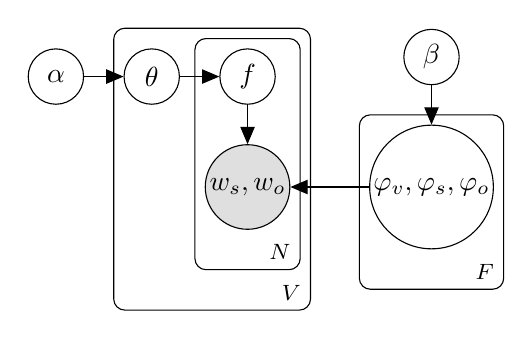
\begin{tikzpicture}[]
    \node[obs]                   (w)     {$w_s,w_o$}; %
    \node[latent, above=0.5cm of w]     (f)     {$f$};
    \node[latent, left=0.5cm of f]     (theta) {$\theta$};
    \node[latent, left=0.5cm of theta] (alpha) {$\alpha$};
    \node[latent, right=of w]    (phi)   {$\varphi_v,\varphi_s,\varphi_o$};
    \node[latent, above=0.5cm of phi] (beta) {$\beta$};
    \edge {alpha} {theta};
    \edge {theta} {f};
    \edge {f} {w};
    \edge {phi} {w};
    \edge {beta} {phi};
    \plate {frames} {(phi)} {$F$};
    \plate {datapoints} {(f) (w)} {$N$};
    \plate {verbs} {(f) (w) (datapoints) (theta)} {$V$};
\end{tikzpicture}


    \caption{Model 1 generative story}
    \label{gen1}

\end{figure}

The independence assumptions in the generative story for model 1 give us the 
following joint distribution:

\begin{align*}
&P(\mathbf{w},\mathbf{f}|\theta,\phi,\alpha,\beta)\\
&=P(\mathbf{w}|\mathbf{f},\phi)\,P(\mathbf{f}|\theta)\,P(\theta|\alpha)\,P(\phi|\beta)
\end{align*}

We can find the marginal distribution of the latent and observed variables by
integrating over the priors:

\begin{align*}
& P(\mathbf{w},\mathbf{f}|\alpha,\beta)\\
&=\int_\phi\int_\theta P(\mathbf{w},\mathbf{f}|\theta,\phi,\alpha,\beta)\\
&=     \int_\phi P(\mathbf{w}|\mathbf{f},\phi )\,P(\phi|\beta)
\times \int_\theta P(\mathbf{f}|\theta)\,P(\theta|\alpha)
\end{align*}

These integrals are both dirichlet multinomials:

\[
\frac{DCM_i^{frames}(f_{ij}=f, \mathbf{f}_{-ij})}{DCM_i^{frames}(\mathbf{f}_{-ij})}
\]

and

\[
\prod_a^{\{v,s,o\}}\frac{DCM_i^{vocab^a}(f_{ij}=f, \mathbf{f}_{-ij})}{DCM_i^{vocab^a}(\mathbf{f}_{-ij})}
\]

We prefer not to consider the subject and object vocabularies independently 
(i.e., $V^s = V^o$). This is more in line with the theory of semantic frames 
since in principle, a noun playing a particlar semantic role may appear in either 
syntactic position.

Dropping terms not dependent on counts, we can calculate the probability 
required for Gibbs sampling as follows:

\begin{align}
& P(f_{ij} = f|\mathbf{f}_{-ij},\mathbf{w}, \alpha,\beta)\nonumber\\
&=\frac{\alpha + \tilde c(d_i,f)}{F\,\alpha + \tilde c(d_i)}
\times \prod_a^{\{v,s,o\}}\frac{\beta+\tilde c(f,w_{ij}^a)}{V^a\beta+\tilde c(f)}
\end{align}

Where $\tilde c (d_i, f)$ is the number of VSO's in document $d_i$ assigned to frame $f$,
$\tilde c(d_i)$ is the number of VSO's in document $i$,
$\tilde c(f,w_{ij}^a)$ is the number of VSOs containing $w_{ij}^a$ as argument $a$ that are
assigned to frame $f$, and
$\tilde c(f)$ is the number of VSOs assigned to frame $f$.
Note that $\tilde c$ indicates a count that does not consider the contribution of 
VSO $w_{i,j}$.

We will see that the data used in this probject doesn't contain any document-level
information. As a result, we adapt model 1 by grouping VSOs with the same verb into ``documents''.
This move leverages the dirichlet prior $\alpha$ to enforce sparcity of frames 
accross verbs, but of course cannot capture the information given by the kind of
document-level semantic sparsity seen in LDA.\footnote{When we use verbs as
documents (i.e, $D = V^v$), since $w_{ij}^v$ is the same for all verbs in document $d_i$ 
(and $d_i$ is the only document with that verb), it follows that the number of VSO's in document 
$d_i$ belonging to frame $f$ is the same as the number of VSO's with $w_{ij}^v$ as their verb assigned to 
frame $f$; that is, $\tilde c(d_i, f) = \tilde c(f, w_{ij}^v)$.}

\section{Data}

\subsection{Google Syntactic-ngrams}
Here we talk a bit about the syntactic n-grams and all that \citep{ngrams2013}.
\begin{itemize}
    \item A syntactic-ngram is a $k$-word rooted subtree for some sentence. 
    \item Google ngrams come from a corpus of 3.5 million English books.
    \item We trimmed the ``verb args'' dataset to consider only subject-verb-object triples (VSO's).
    \item The dataset contains 1,629,120 unique VSO's with a total of 96,245,401 by count.
    \item In our final results we may only use the most common \%20 of these...
\end{itemize}

\subsection{Pruning}


\section{Experiments}


\section{Results}
\subsection{Frame Coherency}
rame coherency: for a datapoint $(v,s,o)$ and a tuple $(v^r,s,o)$ where $v^r$ is a random choses verb: $P(v\mid s,o) \geq P(v^r\mid s,o)$  
\subsection{Frame Correctness}
% I (Eli) can expond here on the relation/contrast/etc.
%   between what we're doing and Framenet;
%   I think O'Connor brings up some technical and/or methodological points
%   about ways we can vs. can't use the FN data for evaluating
%   induction and such, I'll look it over again.

Frame correctness: for the top 25 most probable verbs per frame $TV$ and framenet classes of verbs $FN$: \[\frac{2|TV\cap FN|}{|TV|+|FN|}\]

\subsection{Model 0}
\subsection{Model 1}


\section{Discussion}


\section{Future Work}
\begin{itemize}
\item Come up with models that are specifically for independent tuples.
\item Use more of the arguments in verbargs.
\item Use year information -- do frames change over time?
\item Consider subjet/object pairs instead of independent.
\end{itemize}

\section{Conclusion}


\bibliography{refs.bib}
\end{document}
